
\documentclass[12pt]{article}
\usepackage[utf8]{inputenc}
\usepackage{graphicx}
\usepackage{geometry}
\usepackage{setspace}
%\usepackage{booktabs}
\usepackage{hyperref}
\geometry{margin=1in}
\setstretch{1.2}

\title{The Hidden Costs of Subsidized Housing in Bogotá:\\
Rent vs.\ Buy, Liquidity, and the False Promise of VIS/VIP}
\author{Igor Rivin\\
\small{with assistance from Claude and ChatGPT}}
\date{\today}

\begin{document}
\maketitle

\begin{abstract}
We assemble a twenty-year rent--versus--buy framework for Colombia's VIS/VIP housing and include the frictions that most policy summaries omit: gray-delivery finishing financed at consumer rates, uncovered down payment financed at consumer rates, HOA and maintenance creep, CPI-indexed commuting time, transaction and illiquidity costs, and early-sale clawbacks. Under realistic CPI-linked rents and flat-to-negative real appreciation, we find no scenario in which VIS ownership beats renting within 20 years. To our knowledge, this is the first comprehensive financial analysis comparing total ownership costs to renting for Colombia's VIS program, despite widespread anecdotal evidence of quality issues and subsidy failures.
\end{abstract}

\section*{Methods (key points)}
\begin{itemize}
  \item Down payment requirement 20\%; subsidy covers 10\%; the uncovered 10\% is financed (15\%, 5 years).
  \item Finishing (obra gris): 30M COP, financed (13\%, 5 years).
  \item Mortgage: 20 years at 9\% APR; HOA grows with CPI; maintenance grows at CPI+2\%.
  \item Commuting time valued at CPI-indexed wage; 10 h/wk (central rent) vs 20 h/wk (peripheral own).
  \item Net-if-sold only plotted after 10-year lockup/clawback.
\end{itemize}

\section*{Results}
\subsection*{Dominant scenario (CPI 3\%, nominal appreciation 1\%)}
\begin{figure}[h]
\centering
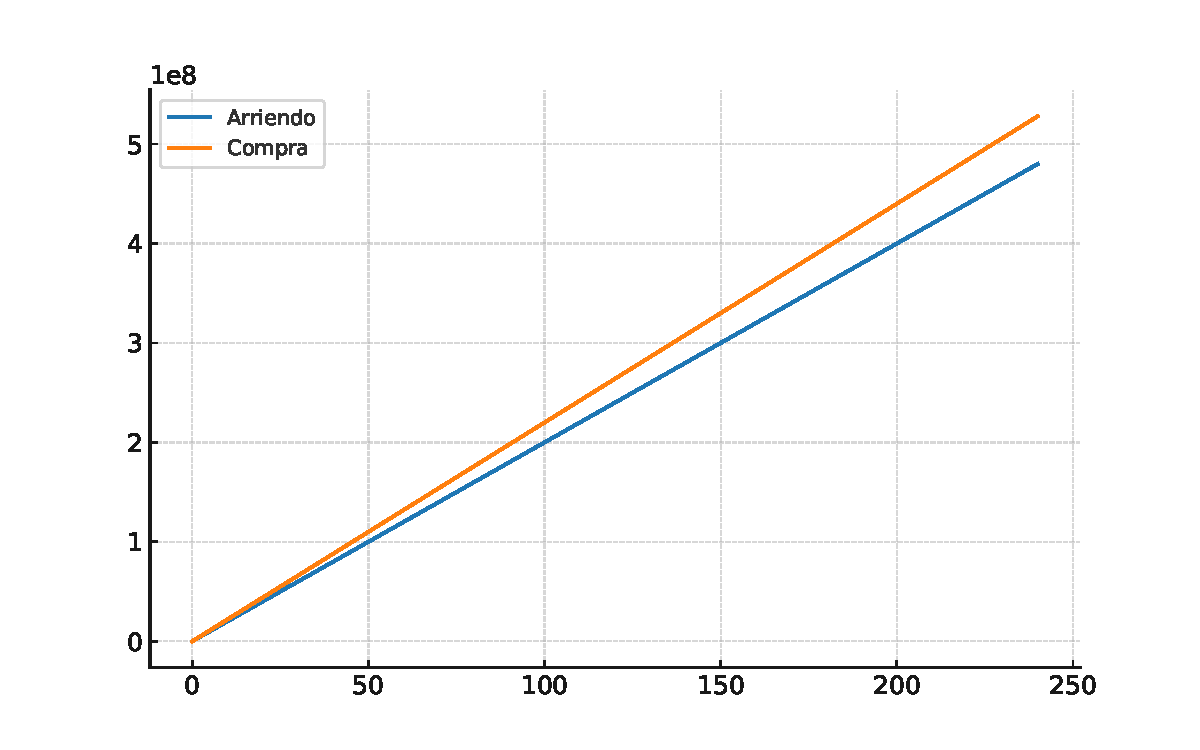
\includegraphics[width=0.9\textwidth]{cash_outflows_dominant.pdf}
\caption{Cumulative cash outflows (rent vs buy), including CPI-indexed time costs.}
\end{figure}

\begin{figure}[h]
\centering
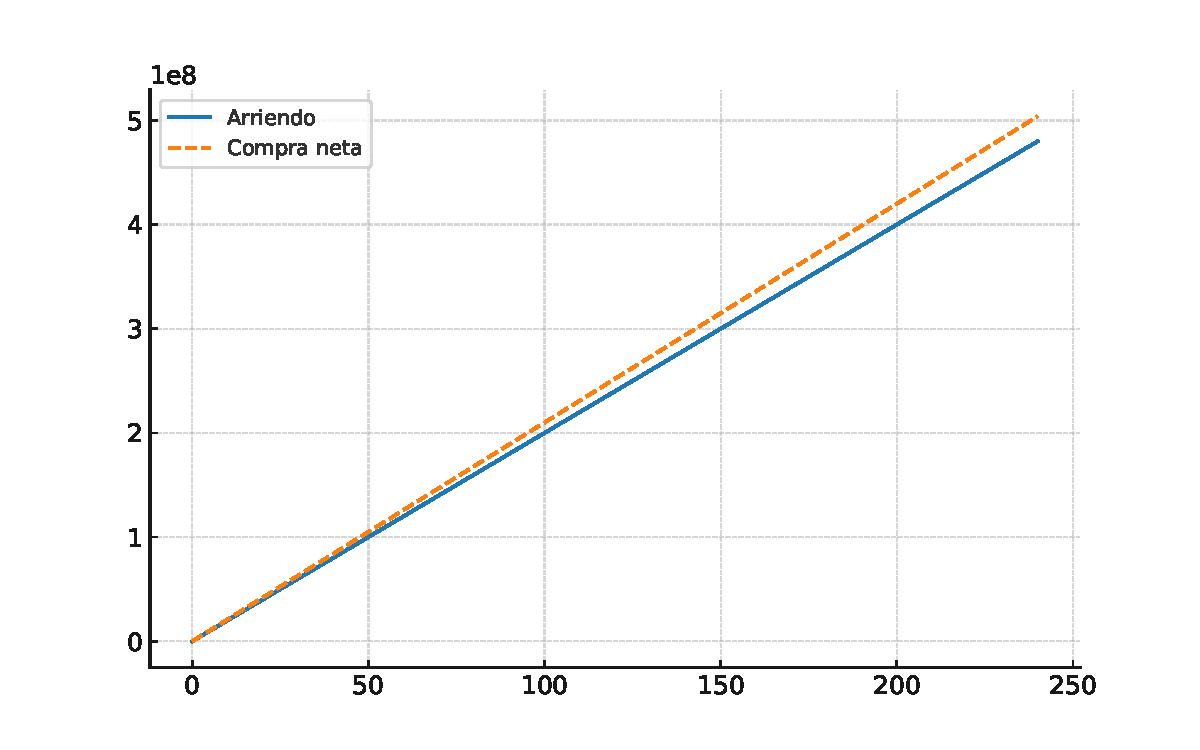
\includegraphics[width=0.9\textwidth]{net_if_sold_dominant.pdf}
\caption{Net position if sold (only after 10-year lockup), compared to rent cumulative.}
\end{figure}

\subsection*{Sensitivity (CPI $\times$ nominal appreciation)}
Below, CPI-paths (1\%, 3\%, 5\%) vs nominal appreciation (0\%, 1\%, 2\%). Values in millions of COP. `Net if sold' only applies after year 10.

\begin{table}[h]
\centering
\small
\begin{tabular}{llrrrrr}
\hline
CPI & Appr & Year & Rent cum (M) & Own cum (M) & Net if sold (M) & Own$-$Rent (M) \\
\hline
1\% & 0\% & 10 & 258.5 & 385.4 & --- & --- \\
1\% & 1\% & 15 & 397.7 & 555.0 & 483.4 & 157.3 \\
1\% & 2\% & 20 & 544.0 & 730.4 & 606.7 & 186.4 \\
3\% & 0\% & 10 & 236.1 & 380.6 & --- & --- \\
3\% & 1\% & 15 & 357.6 & 544.5 & 472.8 & 214.9 \\
3\% & 2\% & 20 & 498.5 & 712.4 & 588.7 & 213.9 \\
5\% & 0\% & 10 & 215.9 & 377.5 & --- & --- \\
5\% & 1\% & 15 & 320.6 & 537.2 & 462.4 & 216.6 \\
5\% & 2\% & 20 & 441.7 & 701.2 & 574.8 & 230.0 \\ \hline
\end{tabular}
\caption{Sensibilidad (CPI 1\%, 3\%, 5\%) vs. apreciaci\'on nominal (0\%, 1\%, 2\%). Valores en millones de COP.}
\label{tab:sensitivity}
\end{table}


\section*{Discussion}
\textbf{No early win:} Owning never dominates within 20 years under realistic CPI/appreciation.\\
\textbf{Overcharge $\rightarrow$ haircut:} VIS units priced at the subsidy ceiling imply resale haircuts in early years (even before fees).\\
\textbf{Engaño of expected appreciation:} Anecdotal success stories (e.g. a house in Cúcuta bought for USD 20k and later valued at USD 40–50k) create the belief that real estate in Colombia 'always doubles.' VIS/VIP periphery projects differ: units are sold at inflated subsidy ceilings, new subsidized supply arrives constantly, and locations like Soacha or Bosa lack scarcity or prestige. Used VIS units must compete with new ones that qualify for subsidies, leading to a saturated market and weak or negative appreciation. Expecting a Cúcuta-style doubling is therefore an engaño. \\

\textbf{Liquidity lock-in:} With lockup+slow resale, moving imposes double housing or a quick-sale discount.\\
\textbf{Time and access:} CPI-indexed commute costs (and loss of access) are first-order for welfare.

\section*{Appendix A (Resumen en Español, con tabla)}
\textbf{Conclusión rápida:} En ningún escenario la compra VIS gana en los primeros 20 años; la mejor diferencia sigue siendo perder alrededor de \textbf{68.1} millones de COP frente al arriendo. Por la sobrevaloración inicial (tope del subsidio), vender en los primeros años casi siempre implica \emph{perder plata} (``haircut''). 

Muchas familias piensan que la vivienda siempre se valoriza, recordando casos como una casa en Cúcuta comprada en 20 mil dólares y luego vendida en 40--50 mil. Pero el caso VIS es distinto: los precios ya arrancan inflados al tope del subsidio, los proyectos nuevos siguen llegando cada año, y las zonas (Soacha, Bosa, Ciudad Bolívar) no son escasas ni prestigiosas. El usado compite con el nuevo que además trae subsidio. El resultado: poca o nula valorización real. Esperar que un apartamento VIS se 'duplique' es un engaño peligroso.

\begin{table}[h]
\centering
\small
\begin{tabular}{llrrrrr}
\hline
CPI & Appr & Year & Rent cum (M) & Own cum (M) & Net if sold (M) & Own$-$Rent (M) \\
\hline
1\% & 0\% & 10 & 258.5 & 385.4 & --- & --- \\
1\% & 1\% & 15 & 397.7 & 555.0 & 483.4 & 157.3 \\
1\% & 2\% & 20 & 544.0 & 730.4 & 606.7 & 186.4 \\
3\% & 0\% & 10 & 236.1 & 380.6 & --- & --- \\
3\% & 1\% & 15 & 357.6 & 544.5 & 472.8 & 214.9 \\
3\% & 2\% & 20 & 498.5 & 712.4 & 588.7 & 213.9 \\
5\% & 0\% & 10 & 215.9 & 377.5 & --- & --- \\
5\% & 1\% & 15 & 320.6 & 537.2 & 462.4 & 216.6 \\
5\% & 2\% & 20 & 441.7 & 701.2 & 574.8 & 230.0 \\ \hline
\end{tabular}
\caption{Sensibilidad (CPI 1\%, 3\%, 5\%) vs. apreciaci\'on nominal (0\%, 1\%, 2\%). Valores en millones de COP.}
\label{tab:sensitivity}
\end{table}


\end{document}
